\subsection{Proportion of individuals within target}\label{sec:proportion_within_target}

Another performance measure that is taken into consideration is the proportion 
of individuals whose time in the hospital (waiting and service time) is within
a specified time target \(t\).
Similar to section \ref{sec:waiting_time}, three formulas are needed for this 
performance measure.

The proportion of type 1 individuals within a time target:

\begin{equation}\label{eq:proportion_within_target_type_1}
    P(X^{(1)} < t) = \frac{\sum_{(u,v) \in S_A^{(1)}} 
    P(X_{\mathcal{A}_1(u,v)}^{(1)} < t) 
    \pi_{u,v} }{\sum_{(u,v) \in S_A^{(1)}} \pi_{u,v}}
\end{equation}

The proportion of type 2 individuals within a time target:

\begin{equation}\label{eq:proportion_within_target_type_2}
    P(X^{(2)} < t) = \frac{\sum_{(u,v) \in S_A^{(2)}} 
    P(X_{\mathcal{A}_2(u,v)}^{(2)} < t) 
    \pi_{u,v} }{\sum_{(u,v) \in S_A^{(2)}} \pi_{u,v}}
\end{equation}

The terms \(\mathcal{A}_1(u,v)\) and \(\mathcal{A}_2(u,v)\) are defined by
equations \ref{eq:arriving_state_class_1} and \ref{eq:arriving_state_class_2}
in section \ref{sec:blocking_time}.
The overall proportion individuals within a time target (where \(P_{L'_1}\) and 
\(P_{L'_1}\) are defined in (\ref{eq:proportion_of_accepting_individuals})):

\begin{equation}\label{eq:overall_proportion_within_target}
    P(X < t) = \frac{\lambda_1 P_{L'_1}}{\lambda_2 P_{L'_2}+\lambda_1 P_{L'_1}} 
    P(X^{(1)} < t) + \frac{\lambda_2 P_{L'_2}}{\lambda_2 P_{L'_2} + 
    \lambda_1 P_{L'_1}} P(X^{(2)} < t) 
\end{equation}

Here \(P(X_{(u,v)}^{(1)})\) and \(P(X_{(u,v)}^{(2)})\) are defined as the
proportion of individuals within the time target \(t\) when starting from state 
\((u,v)\).
These expression can be calculated by:

\begin{equation}\label{eq:proportion_within_target_type_1_from_state}
    P(X_{(u,v)}^{(1)} < t) = 
    \begin{cases}
        1 - \sum_{i=0}^{v-1} \frac{1}{i!} e^{-\mu t} (\mu t)^i, 
            & \textbf{if } C = 1 \\
            & \textbf{and } v>1 \\
        1 - (\mu C)^{v-C} \mu  
            \sum_{k=1}^{\mid \vec{r} \mid} \sum_{l=1}^{r_k}
            \frac{\Psi_{k,l}(-\lambda_k)t^{r_k - l} 
            e^{-\lambda_k t}}{(r_k - l)! (l - 1)!},
            & \textbf{if } C > 1 \\
            & \textbf{and } v > C \\
        1 - e^{-\mu t},  & \textbf{if } v \leq C
    \end{cases}
\end{equation}

\noindent
where \(\vec{r}=(v - C, 1)\), \(\vec{\lambda}=(C \mu, \mu)\) and 
\(\lambda_0 = 0, r_0\) = 1. 

\begin{equation}\label{eq:proportion_within_target_type_2_from_state}
    P(X_{(u,v)}^{(2)} < t) = 
    \begin{cases}
        1 - \sum_{i=0}^{\min(v,T)-1} \frac{1}{i!} e^{-\mu t} (\mu t)^i,  
            & \textbf{if } C = 1 \\ 
            & \textbf{and } v, T > 1 \\
        1 - (\mu C) ^ {\min(v,T) - C} \mu  
        \sum_{k=1}^{\mid \vec{r} \mid} & \textbf{if } C > 1 \\
        \qquad \times \sum_{l=1}^{r_k}
        \frac{\Psi_{k,l}(-\lambda_k)t^{r_k - l} 
        e^{-\lambda_k t}}{(r_k - l)! (l - 1)!}, 
            & \textbf{and } v, T  > C\\
        1 - e^{-\mu t}, & \textbf{if } v \leq C \\ 
            & \textbf{or } T \leq C \\
    \end{cases}
\end{equation}

\noindent
where \(\vec{r}=(\min(v, T) - C, 1)\), \(\vec{\lambda}=(C \mu, \mu)\) and
\(\lambda_0 = 0, r_0 = 1\).


The function \(\Psi_{k,l}\) used in equations 
(\ref{eq:proportion_within_target_type_1_from_state}) and 
(\ref{eq:proportion_within_target_type_2_from_state}) is defined as:

\begin{equation}
    \Psi_{k,l}(t) = 
    \begin{cases} 
        \frac{(-1)^{l} (l-1)!}{\lambda_2} \left[\frac{1}{t^l} - \frac{1}
        {(t + \lambda_2)^l}\right] , & k=1 \\
        - \frac{1}{t (t + \lambda_1)^{r_1}}, & k=2
    \end{cases} \nonumber \\
\end{equation}

Please refer to appendix \ref{sec:appendix_mean_proportion} for a more in-depth 
explanation of the origins of equations 
(\ref{eq:proportion_within_target_type_1}) - 
(\ref{eq:proportion_within_target_type_2_from_state}).

Figure \ref{fig:markov_vs_des_proportion_comparison_overall} shows a comparison
of the mean proportion of individuals within target when using Markov chains 
and discrete event simulation (appendix~\ref{sec:appendix_des}).
The figure is used to demonstrate the accuracy of the formula for the 
proportion of individuals within time of the constructed queueing model
as well as the effect that truncating the model has on the formula.
The simulation was run 100 times and the recorded proportions at each iteration 
is used to populate the violin plots.
Similar to figures \ref{fig:markov_vs_des_waiting_time_comparison_overall} and
\ref{fig:markov_vs_des_blocking_time_comparison}, these plots shows a comparison
between the calculated mean proportion of individuals within time using Markov 
chain, using a truncated simulation and using a simulation 
without the artificial parameters \(N\) and \(M\).
The proportions generated by the truncated simulation match the ones generated
by the Markov chains model.
Note that this comparison includes both type 1 and type 2 individuals.
A separate comparison of only type 1 and only type 2 individuals can be found 
in appendix~\ref{sec:appendix_additional_figures}.

\begin{figure}[H]
    \centering
    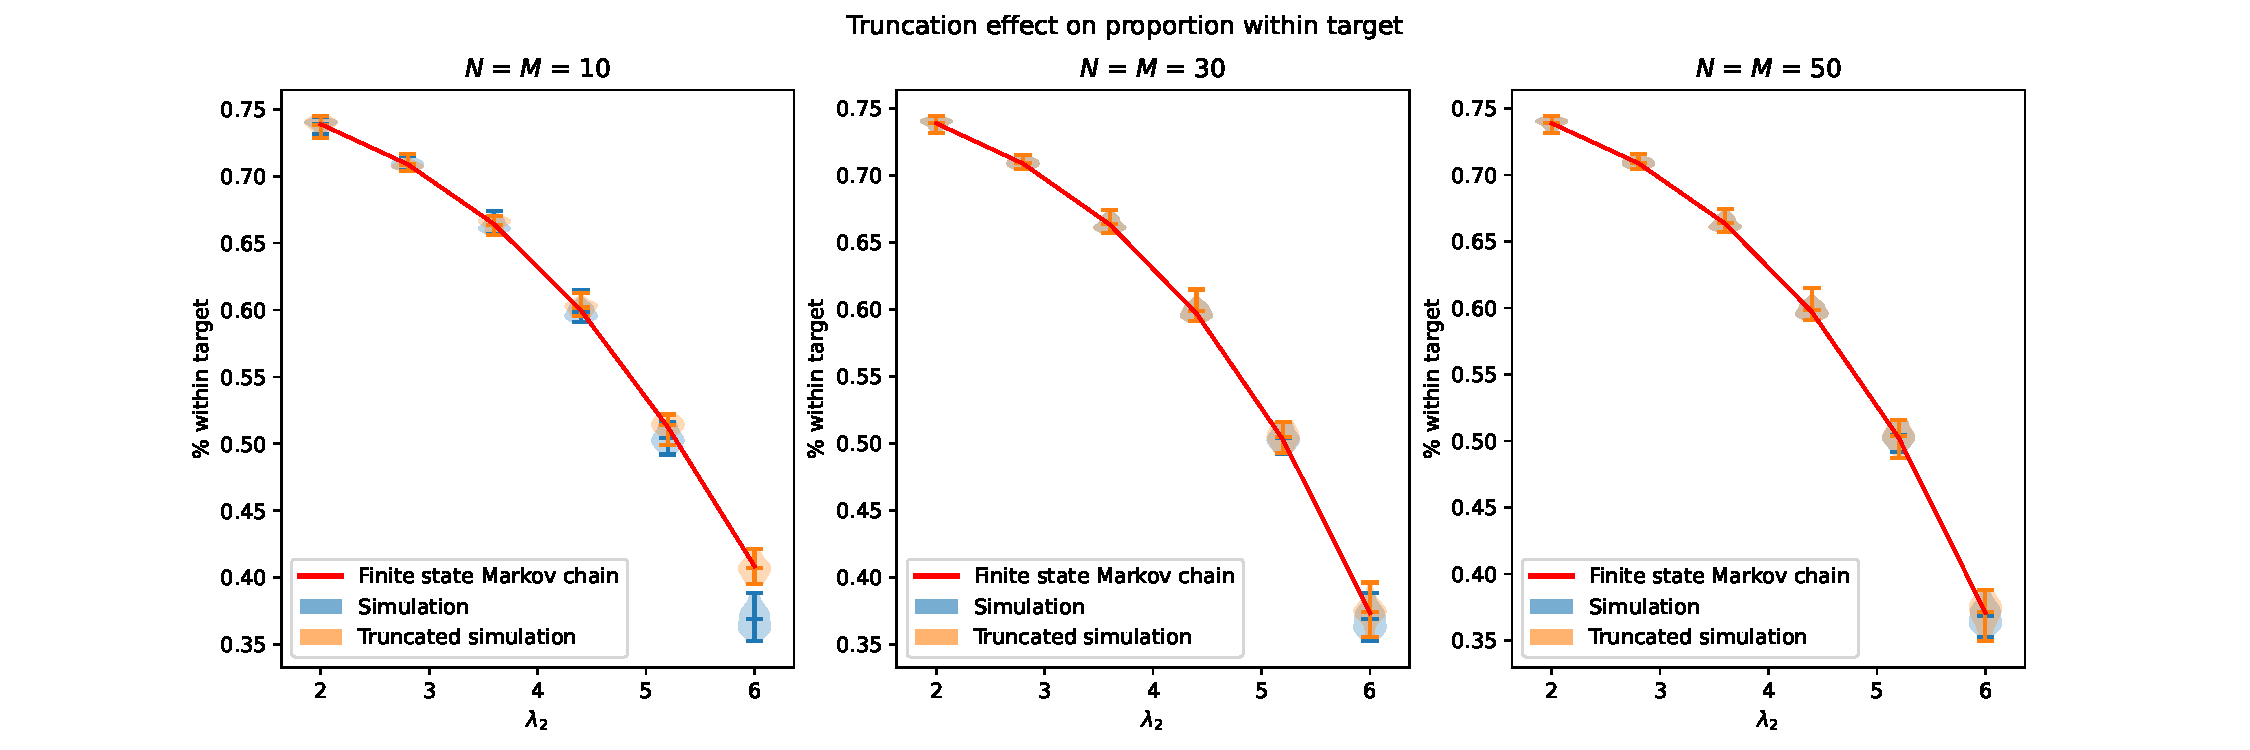
\includegraphics[width=\textwidth]{imgs/truncation_effect/proportion/main.pdf}
    \caption{
        Comparison of mean proportion of individuals within target time between 
        values obtained from the Markov chain formula, values obtained from the
        truncated simulation and values obtained from the untruncated
        simulation. 
    }
    \label{fig:markov_vs_des_proportion_comparison_overall}
\end{figure}
